%\chapter{Procedimentos metodológicos}
\label{Metodologia}

%	\begin{flushright}
%		\textit{``Um bom começo é a metade''.\\
%		Aristóteles}
%	\end{flushright}


%A presente pesquisa é descritiva, aplicada e experimental, para a qual foi necessário: i) coletar e reunir uma massa de dados convencional de empresa, com diferentes tipos de documentos, idiomas e gêneros linguísticos; ii) projetar e implementar um arcabouço de \textit{software} que indexou a massa de dados de documentos corporativos usando uma estrutura de dados, e fez o reconhecimento de termos e sua consequente associação a facetas através de dicionários, \textit{gazetteer}, e de outros bancos de dados acessórios; iii) projetar o primeiro cenário de avaliação baseado naqueles existentes no \textit{framework} TREC, utilizando-se da massa de dados do \textit{framework}; iv) investigar o segundo cenário de avaliação baseado em expressões de busca dos usuários de informação da coleção particular construída para este trabalho; v) estudar e comparar o desempenho das técnicas propostas através das métricas adotadas no TREC; vi) produzir anotações na massa de dados própria como proposta para avaliação de técnicas de recuperação de informação corporativa em conjuntos heterogêneos de documentos quanto ao tipo, idioma e gênero linguístico.

%\textbf{Introdução das etapas metodológicas.}
Está pesquisa é descritiva em se tratando dos objetivos, já que tem como objetivo descrever as características observadas do objeto de pesquisa. É aplicada do ponto de vista de sua natureza, considerando que busca contrastar os resultados obtidos em modelos teóricos e simulações com resultados medidos em uma implementação real. É classificada como qualitativa quanto à abordagem ao problema, pois os resultados apresentados são medições de grandezas do objeto de estudo.

Os procedimentos metodológicos são organizados nas seguintes etapas: 

\begin{enumerate}

\item reunir e estudar os principais trabalhos de organização de informação, especialmente aqueles orientados a coleções corporativas -- parte da pesquisa que pode ser classificada como bibliográfica e tornou-se fundamental para reconhecer características do domínio corporativo que já foram explicitadas por outros autores, de diversas áreas do conhecimento;

\item reunir dois exemplares do domínio corporativo, sendo que um deles é uma coleção pública, altamente reconhecida na literatura; e o outro é uma coleção particular criada especificamente para o trabalho desta tese, resultado da coleta e reunião de uma massa de dados convencional de uma empresa, com diferentes tipos de documentos, idiomas e gêneros linguísticos -- parte da pesquisa que pode ser classificada como pesquisa documental;

\item propor um conjunto mínimo de facetas que represente a informação corporativa das duas empresas investigadas -- parte da pesquisa que pode ser classificada como pesquisa documental; 

\item projetar e implementar um arcabouço de \textit{software} que indexe a massa de dados de documentos corporativos usando estruturas de dados específicas -- parte da pesquisa que pode ser classificada como estudo de caso;

\item avaliar os resultados usando as expressões de busca dos usuários da informação para recuperar documentos da coleção particular -- parte da pesquisa que pode ser classificada como levantamento;

\item avaliar o desempenho da organização facetada utilizando-se do método de avaliação de Cranfield, observando os resultados da trilha \textit{Enterprise} da \textit{Text Retrieval Conference} (TREC) -- parte da pesquisa que pode ser classificada como pesquisa experimental;

\item preparar a coleção particular para que sirva como proposta para avaliação de técnicas de recuperação de informação corporativa em conjuntos heterogêneos de documentos quanto ao tipo e gênero textual, em língua portuguesa -- parte da pesquisa que pode ser classificada como pesquisa participante.

\end{enumerate}

%\textbf{Link para as seções e para a figura.}
As diferentes etapas são descritas mais detalhadamente nas próximas seções do presente capítulo e sintetizadas na figura \ref{fig:metodologia}. %Pela observação da figura o processo de pesquisa parece linear, da revisão de literatura até a disponibilização da coleção particular. As diferentes etapas dos procedimentos metodológicos serão explicadas nas próximas seções.
%No entanto, o processo sofre reflexos da aplicação da análise facetada e da prototipação de \textit{software}, tornando-se iterativo em algumas ocasiões. 


\section{Revisão da literatura}

%\textbf{2 conjuntos da revisão: trabalhos relacionados; bases de comparação da avaliação experimental}
A revisão de literatura empregada neste trabalho resulta em dois conjuntos distintos de trabalhos relacionados: i) a revisão do estado da arte em análise de domínio e recuperação de informação; e ii) o levantamento bibliográfico dos principais resultados de trabalhos anteriores que explicitaram características do domínio corporativo, com origem em diversas áreas do conhecimento.%, encerrado após a conclusão da análise preliminar de domínio.

\begin{figure}
	\caption{\label{fig:metodologia}Procedimentos metodológicos}

	\centering
		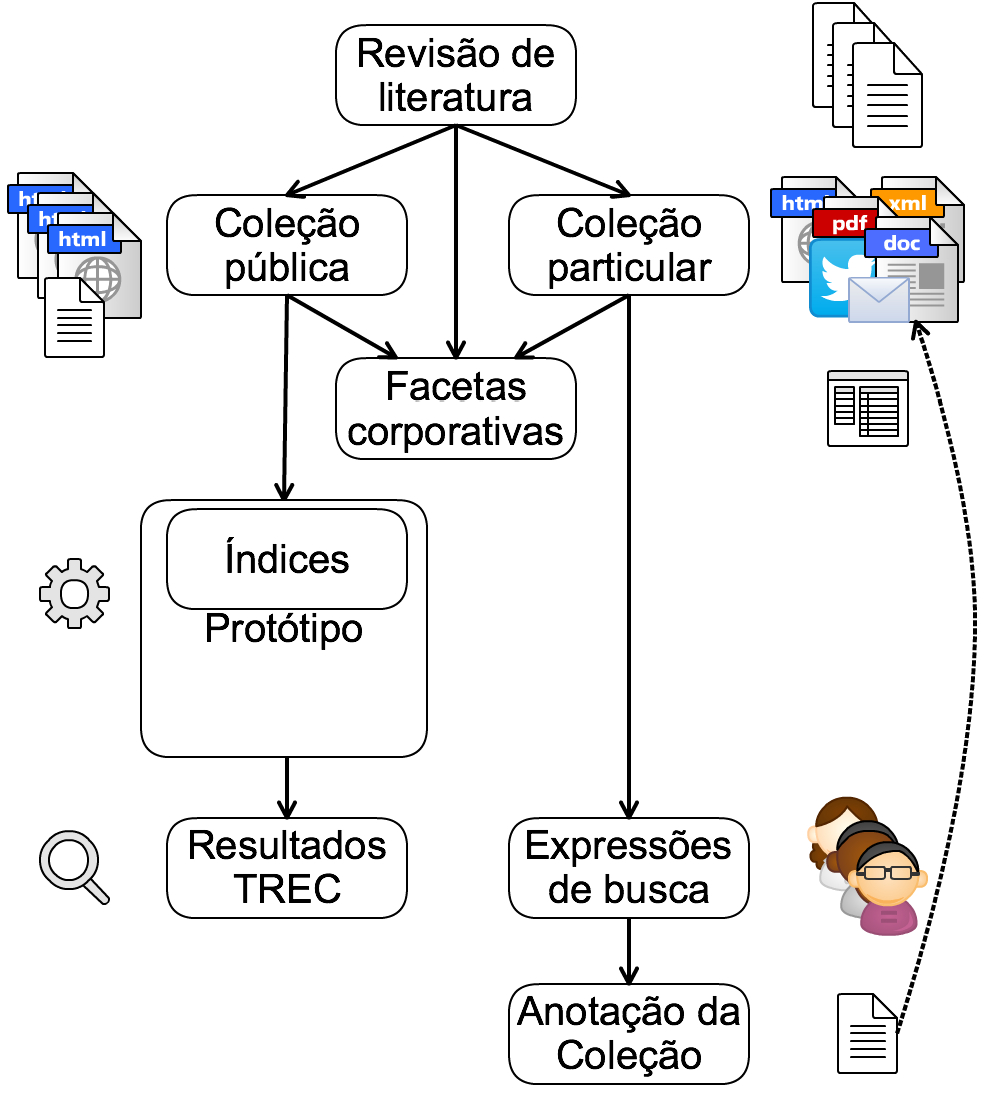
\includegraphics[width=.80\textwidth]{fig/metodologia.jpg}

	\legend{Fonte: elaborada pelo autor}
\end{figure}

%\textbf{Onde encontrar o primeiro conjunto.}
O estado da arte e da técnica em análise de domínio e recuperação da informação é apresentado no capítulo \ref{literatura}. O contexto corporativo foi adotado para limitar o escopo deste trabalho e torná-lo viável para estudos com usuários e para classificação intelectual de documentos. Com isso, trabalhos relacionados mais especificamente à informação corporativa são especialmente de interesse. Na literatura sobre informação corporativa, também se busca um conjunto de facetas para a informação corporativa, como se observa na figura \ref{fig:metodologia}. Características da informação corporativa naturalmente permeiam os produtos tecnológicos de recuperação de informação corporativa e são discutidas em trabalhos sobre o tema nas áreas de Ciência da Computação e Biblioteconomia e Ciência da Informação. Entretanto, a fragmentação desse conhecimento torna difícil produzir um mapa das características do domínio corporativo. Adicionalmente, como os trabalhos tendem a assumir uma perspectiva mais pragmática, as características corporativas já conhecidas tendem a ser úteis e restritas apenas ao seu contexto original de estudo.

%\textbf{Onde encontrar o segundo conjunto.}
O segundo produto da revisão engloba um conjunto com os principais métodos automáticos e semiautomáticos de classificação, indexação e \textit{ranking} de informação, bem como as métricas usadas para avaliação experimental do desempenho dos métodos. Devidamente estudados, devem servir de base de comparação para projetar métodos mais adequados para organizar e recuperar informação corporativa. O segundo produto é apresentado na seção \ref{prototipo-colecaoPublica}, precisamente onde é adotado para validar os resultados deste trabalho sobre a coleção pública.

%Tais métodos foram implementados dentro do \textit{software} de gerenciamento de bibliotecas digitais como parte da prototipação.

\section{Coleções de documentos}

%\textbf{2 coleções.}
Neste trabalho, duas coleções de documentos corporativos são adotadas para a análise de domínio. A primeira coleção refere-se à coleção de referência usada na trilha \textit{Enterprise} da \textit{Text Retrieval Conference} (TREC) até o ano de 2008. Trata-se de uma coleção de 370.715 páginas \textit{Web} públicas da \textit{Commonwealth Scientific and Industrial Research Organisation} (CSIRO). A segunda coleção refere-se a um conjunto mais amplo de documentos, o que inclui atas, relatórios, memorandos, e-mails e páginas \textit{Web} públicas.

%\textbf{uma coleção é pública.}
A coleção de referência da \textit{Text Retrieval Conference} é útil por facilitar a comparação entre experimentos empíricos relatados na literatura e experimentos empreendidos nesta tese. Porém, seu uso tem sido criticado por contar exclusivamente com páginas \textit{Web} pública da CSIRO, criando condições que em nada se parecem com aquelas presentes em um ambiente real de busca corporativa. %A caracterização desta coleção é apresentada na seção 4.1.%Considerações de outros autores sobre seu uso e sobre metodologias de avaliação serão apresentadas na seção \ref{avaliacao}.

%\textbf{uma coleção é particular.}
Na tentativa de reduzir as limitações da coleção de referência, é adotada uma segunda coleção de documentos. Trata-se de um conjunto de documentos de uma empresa pública brasileira, com uma diversidade maior de tipos de documentos que aquela encontrada na coleção de referência. Ela se caracteriza como um ambiente mais próximo da realidade de uma empresa e das necessidades de informação de um usuário corporativo real, porém não pode ser vista como uma substituta da coleção de referência da \textit{Text Retrieval Conference} e nem mesmo como uma coleção perfeita para todo e qualquer objetivo. Nesta tese, a segunda coleção é denominada como coleção particular. No entanto, a coleção também se tornará publicamente disponível no ano de 2015. %A caracterização da nova coleção é apresentada na seção 4.2.%A segundo coleção de documentos foi concluída antes mesmo que a revisão da literatura fosse encerrada. 

%\textbf{Classificação de tarefas de buscas Versus Presença de usuários reais.}
Documentos da coleção pública são classificados para diferentes tarefas de busca. As tarefas de busca são aquelas mais comumente realizadas por usuários de informação reais, responsáveis pela classificação intelectual dos documentos para a avaliação, sendo que os usuários não são conhecidos. Ao contrário, para estudos sobre a coleção particular está disponível uma amostra de usuários reais.

%\textbf{2 experimentos.}
A presença de duas coleções provoca impactos em vários procedimentos metodológicos, como a figura \ref{fig:metodologia} ilustra, requerendo dois experimentos e avaliações diferentes. Enquanto a coleção particular faz uso de seus usuários para validar os resultados deste trabalho, a coleção pública conta com resultados prévios obtidos em duas edições da \textit{Text Retrieval Conference}, em 2007 e 2008.

%\textbf{Validação das coleções.}
Finalmente, a coleção particular tem sido usada por seus usuários para a realização de trabalho e para a tomada de decisão nos últimos anos. Portanto, partindo do pressuposto que a coleção particular seja uma coleção corporativa válida, pretende-se validar também a coleção pública como uma coleção corporativa ao demonstrar a compatibilidade de ambas.

\section{Definição de um conjunto mínimo de facetas corporativas}

%\textbf{Técnicas usadas.}
O estabelecimento de um conjunto mínimo de facetas, que possa atender adequadamente as necessidades de diferentes empresas, requer uma análise de domínio. A partir das duas coleções citadas na seção anterior, a análise de domínio adota as técnicas de análise de assuntos e de análise facetada. Ambas as técnicas servem ao propósito de descobrir características dos documentos corporativos e propor um conjunto de facetas comuns a ambas as coleções.

%\textbf{Motivação da adoção da análise facetada para executar a análise de domínio.}
A análise facetada permite ampliar facilmente esse conjunto de características, a\-co\-mo\-dan\-do-as em esquemas classificatórios hospitaleiros. Isso é útil para permitir que um esquema classificatório mais generalista seja personalizado para uma empresa específica, ou para uma unidade organizacional específica. Por outro lado, um conjunto genérico e realmente expressivo de características é útil para a interoperabilidade entre sistemas de informação, para o intercâmbio de informação corporativa, e principalmente para o projeto mais eficiente de sistemas de recuperação de informação corporativa.%Embora a organização facetada permita facilmente ampliar este conjunto, espera-se que toda a avaliação se concentre em um núcleo pequeno de características, mas de diferentes facetas.

%\textbf{Onde encontrar o conjunto de facetas.}
Os procedimentos metodológicos do processo de análise de domínio, através da análise de assunto e da análise facetada, são descritos no capítulo \ref{analiseDominio}.

%Facetas correspondentes a nomes podem ser facilmente estendidas para nomes de pessoas (funcionários, clientes e colaboradores) e de outras empresas (clientes, fornecedores e subsidiárias). Facetas correspondentes a locais incluem endereços dos diversos atores socio-técnicos existentes, os quais também possuem nomes. Finalmente, facetas relacionadas a tempo referem-se a datas de nascimento, fundação ou inauguração, ocorrência de atendimentos e de publicação de documentos, dentre outras. Outras facetas podem depender de uma combinação ou sobreposição de duas ou três das facetas citadas anteriormente, como é o caso daquelas relacionadas a processos.

%\textbf{Limitação do escopo da análise de domínio.}
%A análise de domínio empreendida corresponde a uma tentativa preliminar. O conjunto de facetas resulta de uma análise de domínio preliminar, inicialmente partindo da revisão da literatura e dos dois exemplares do domínio, citados na seção anterior. O estudo de exemplares do domínio serve para que características da linguagem, adotada por diferentes atores sociais, sejam explicitadas. 

%Os trabalhos encontrados na literatura indicam que muita atenção é dada às entidades que se encontram explícitas nas mensagens entre atores sociais que se comunicam por meio de linguagens técnicas específicas, tais como financeira, jurídica, de informática, de engenharia ou de \textit{marketing}. Mesmo dentro da mesma empresa, entidades são tratadas sob perspectivas muito diferentes dentro das linguagens técnicas específicas, apresentando facetas muito particulares de interesse. Pela análise facetada, são descobertas as facetas dessas entidades que permeiam a maioria ou totalidade das linguagens técnicas específicas. Essas facetas têm o potencial de representar as expressões de busca dos usuários corporativos e de representar minimamente as entidades que são citadas em documentos corporativos, compondo índices de sistemas de recuperação de informação assim como também foi ilustrado na figura \ref{fig:metodologia}. 

\section{Prototipação de um sistema de recuperação de informação corporativa}

%\textbf{Experimento empírico via protótipo.}
A prototipação baseada em \textit{software} é descrita na figura \ref{fig:metodologia} apenas como protótipo. O protótipo de um sistema de recuperação de informação, implementado em linguagem Java e usando a biblioteca Lucene, executa as funções de indexar e recuperar documentos apenas da coleção pública para realizar um experimento empírico. O protótipo é documentado no capítulo \ref{prototipo}.

%\textbf{Metodologia de prototipação.}
A metodologia de prototipação se baseia no trabalho de \citeonline{anastacio09}, pela adoção de mecanismos comuns de coleta, classificação, indexação, busca e recuperação de documentos e sua adaptação para necessidades especiais. No contexto desta tese, os requisitos do protótipo são: organização facetada, tratamento espaço-temporal, e reconhecimento de entidades sociais, espaciais e temporais. Pela implementação desses requisitos, um sistema de recuperação de informação comum torna-se um sistema de recuperação de informação corporativa e facetada.

%\textbf{Requisitos não-funcionais e funcionais.}
Os requisitos não-funcionais do protótipo incluem o tratamento geográfico através da indexação espacial e da implementação de um \textit{gazetteer}; o tratamento temporal através da indexação de indicadores de tempo; e a federação dos repositórios corporativos através da extração de texto dos documentos coletados e a geração de um índice centralizado. Os requisitos funcionais do protótipo corporativo e facetado incluem a indexação, a interface de busca com o usuário, a busca em lote para avaliação de várias expressões de busca em conjunto, e a recuperação de informação.

%\textbf{Requisitos não considerados.}
O controle de acesso a documentos, um importante requisito não-funcional dos sistemas de recuperação de informação corporativa, não é considerado pela natureza da coleção de documentos da CSIRO, constituída apenas por dados acessíveis a todos os usuários. Os efeitos dessa omissão não afetam o cenário de avaliação proposto pela trilha \textit{Enterprise} da \textit{Text Retrieval Conference}. %e nenhum trabalho da literatura parece incorporar esse requisito.

%\textbf{Método experimental se aplica apenas à coleção pública.}
Essa avaliação baseada em prototipação constitui um importante método de validação de resultados desta tese. Porém, sua utilidade é limitada apenas a uma das duas coleções de documentos adotadas, como se observa na figura \ref{fig:metodologia}. A validação de resultados da coleção particular se dá através dos usuários de informação e não beneficia-se diretamente desse método experimental.


%Quais os requisitos mínimos devem ser respeitados para coleta, \textit{parsing}, reconhecimento e desambiguação de facetas, indexação, busca, processamento de consulta, ranking e apresentação?

%iv) Projetar e implementar componentes do SRI corporativo para oferecer suporte a organização facetada da informação, a saber: espaço, tempo, remetente, destinatário, assunto e outras facetas já estudadas por \citet{pontesLima2012, maculan2011, anastacio09} e por \citet{cardosoSantos08}.

%Geo está ok. Quais outras facetas? Como implementar? O que será preciso estudar? Há certeza sobre todas as facetas disponíveis?

\section{Avaliação e validação}

%\textbf{2 cenários de avaliação.}
Dois cenários de avaliação são adotados e ilustrados na figura \ref{fig:metodologia}. O primeiro cenário de avaliação refere-se à avaliação experimental da trilha \textit{Enterprise} da \textit{Text Retrieval Conference}, pela comparação dos resultados desta tese com aqueles de outros trabalhos disponíveis na literatura. Os principais resultados experimentais foram publicados no ano de 2008, quando a trilha foi extinta. O segundo, por sua vez, refere-se exclusivamente à coleção particular e baseia-se em seus usuários. Esse cenário de avaliação usa as expressões de busca elaboradas pelos usuários de informação para avaliar se as características da informação corporativa são reconhecidas por seus usuários. 

%\textbf{Onde encontrar a avaliação.}
Os métodos de avaliação e validação são detalhados no capítulo \ref{prototipo}, juntamente com os resultados da avaliação, sua análise e discussões.

%Usuários da segunda coleção foram empregados no projeto e na execução da segunda avaliação.

%Na coleção privada a avaliação será projetada exclusivamente para este trabalho, por reconhecimento prévio manual de relevância sobre um número reduzido de necessidades informacionais. Espera-se verificar diferentes métricas de desempenho para o processamento de consulta sobre busca em texto completo, busca em metadados, busca em taxonomia facetada classificada intelectualmente e em taxonomia facetada classificada automaticamente a partir de texto completo. A taxonomia facetada refere-se a uma taxonomia criada especificamente para as coleções após a leitura dos documentos. 

\section{Anotação da coleção particular}

%\textbf{Caracterização da coleção particular.}
A coleção pública de documentos, ou coleção de referência, conta com anotações feitas por especialistas. Tais anotações referem-se a caracterização da coleção, listagem de documentos e pessoas relevantes, e de buscas mais frequentes. A coleção particular, usada primeiramente nesta tese, necessita desse tipo de caracterização para ser usada em futuros trabalhos sobre organização da informação corporativa.

%\textbf{Importância da anotação.}
Como demonstrado na figura \ref{fig:metodologia}, a atividade de anotação dessa coleção é realizada a partir da documentação do experimento sobre a coleção particular, constituindo o último produto desta tese. Após a disponibilização de uma réplica da coleção particular, por seus proprietários, a coleção e a sua anotação garantem que os resultados desta tese podem ser repetidos e validados em trabalhos futuros.

%Portanto, a coleção particular torna-se disponível para a comunidade científica apenas após o encerramento deste trabalho, quando os detentores de direitos sobre a coleção particular passam a conhecer os assuntos descobertos em seus próprios dados.


%\textbf{Disponibilização da }
%Uma réplica da coleção particular deve tornar-se pública após uma análise cuidadosa de aspectos relacionados à propriedade intelectual, propriedade industrial e dados sensíveis, sendo fundamental para trabalhos futuros.


%Amazon Turk será usado? O que será manual e o que será automático? Qual o \% de acerto? Precisão! Quanto de cobertura? Revocação! Quanto à busca e ao processamento de consulta, o que combinar? Como? Comparar taxonomia facetada vs taxonomia dinâmica vs fulltext estatístico vs fulltext multifacetado. Qual critério? Precisão? Revocação? Tempo? Side by side? Tarefas trec?

%Tarefas TREC serão comparadas pelos resultados disponibilizados na literatura. Outras tarefas serão comparadas por trabalhos prévios sobre taxonomia facetada de \citet{maculan2011}, para a BDTD da ECI/UFMG, sobre 41 documentos, e taxonomias dinâmicas de \citet{pontesLima2012} para a mesma BDTD.


%A metodologia proposta para esta pesquisa é principalmente experimental, para qual é necessário: i) coletar e reunir uma massa de dados convencional da Web, com diferentes tipos de documentos, idiomas e gêneros linguísticos; ii) projetar e implementar um arcabouço de \textit{software} que indexe a massa de dados de páginas Web usando uma estrutura de dados geométricos, e faça o reconhecimento de topônimos através de um \textit{gazetteer} e das referências geográficas da própria massa de dados indexada; iii) projetar o primeiro cenário de avaliação baseado naqueles existentes no \textit{framework} GeoCLEF, utilizando-se da massa de dados do \textit{framework}; iv) projetar o segundo cenário de avaliação baseado na massa de dados construída para este trabalho; v) estudar e comparar o desempenho das técnicas propostas com os indicadores apresentados no GeoCLEF; vi) produzir anotações semiautomáticas na massa de dados própria como proposta para avaliação de técnicas de RIG em conjuntos heterogêneos de documentos quanto ao tipo, idioma e gênero linguístico.

%
%
%\section{Planejamento das atividades}
%\label{planejamento}
%
%O cronograma ilustrado na figura \ref{fig:cronograma} apresenta as próximas atividades necessárias para a implementação deste projeto. O cronograma apresenta apenas as atividades entre fevereiro de 2013 e fevereiro de 2014. O início do período corresponde exatamente ao início da elaboração deste texto, embora procedimentos metodológicos importantes tenham acontecido antes. As atividades estão correlacionadas a capítulos da tese, alguns já presentes neste projeto.
%
%\begin{figure}
%
%	\caption{\label{fig:cronograma}Cronograma}
%
%	\centering
%		\includegraphics[width=1.00\textwidth]{fig/cronograma.jpg}
%	\legend{Fonte: elaborada pelo autor}
%\end{figure}
%


%\begin{center}
%\setlength{\tabcolsep}{0.0mm}
%\renewcommand{\arraystretch}{1.25}
%\begin{tabular}{|l|p{\constlen}||p{\constlen}|p{\constlen}||p{\constlen}|p{\constlen}||p{\constlen}|p{\constlen}||p{\constlen}|}
%\cline{2-9}
%\multicolumn{1}{c}{} & \multicolumn{1}{|c||}{\textbf{2010}} & \multicolumn{2}{|c||}{\textbf{2011}} & \multicolumn{2}{|c||}{\textbf{2012}} & \multicolumn{2}{|c||}{\textbf{2013}} & \multicolumn{1}{|c|}{\textbf{2014}} \\ \hline
%~{\textbf{Tarefas}} &\mk{\textbf{2S}}&\mk{\textbf{1S}}&\mk{\textbf{2S}}&\mk{\textbf{1S}}&\mk{\textbf{2S}}&\mk{\textbf{1S}}&\mk{\textbf{2S}}&\mk{\textbf{1S}} \\ \hline
%~Disciplinas &\pl{3} & & & & & & & \\ \hline
%~Estágio de docência & & & & & \pl{2} & & & \\ \hline
%~Ajustes de reopção  & & & & & \pl{2} & & & \\ \hline
%~Projeto de Tese     & & & & \pl{1} & & & & \\ \hline
%~Execução da Pesquisa& & & & \pl{4} & & & & \\ \hline
%~Escrita da Tese{~} & & & & & & \pl{2} & & \\ \hline
%~Defesa da Tese & & & & & & & & \pl{1}  \\ \hline
%~Produção de Artigos & & & & & \pl{1} & & \pl{2} & \\ \hline
%~Período no DCC & \pl{3} & & & & & & & \\ \hline
%~Período na ECI & & & & \pl{5} & & & & \\ \hline
%\end{tabular}
%\end{center}





